\documentclass[10pt,letterpaper]{article}
\usepackage[utf8]{inputenc}
\usepackage{amsmath}
\usepackage{amsfonts}
\usepackage{amssymb}
\usepackage{graphicx}
\usepackage[left=1.00in, right=1.00in, top=1.00in, bottom=1.00in]{geometry}

\title{Neural networks and physical systems with emergent collective computational abilities}
\author{John J. Hopfield}
\date{January 15, 1982}

\begin{document}
	\maketitle
	
	\begin{abstract}
		Computational properties of use to biological organisms or to the construction of computers can emerge as collective properties of systems having a large number of simple equivalent components (or neurons). The physical meaning of content-addressable memory is described by an appropriate phase space flow of the state of a system. A model of such a system is given, based on aspects of neurobiology but readily adapted to integrated circuits. The collective properties of this model produce a content-addressable memory which correctly yields an entire memory from any subpart of sufficient size. The algorithm for the time evolution of the state of the system is based on asynchronous parallel processing. Additional emergent collective properties include some capacity for generalization, familiarity recognition, categorization, error correction, and time sequence retention. The collective properties are only weakly sensitive to details of the modeling or the failure of individual devices.
	\end{abstract}
	
	\section{Introduction}
	Given the dynamical electrochemical properties of neurons and their interconnections (synapses), we readily understand schemes that use a few neurons to obtain elementary useful biological behavior \cite{willows1973neuronal,kristan1980generation}.
	
	\section{The general content-addressable memory of a physical system}
	Suppose that an item stored in memory is ``H. A. Kramers \& G. H. Wannier \textit{Phys. Rev.} \textbf{60}, 252 (1941)." A general content-addressable memory would be capable of retrieving this entire memory item on the basis of sufficient partial information. The input ``\& Wannier, (1941)" might suffice. An ideal memory could deal with errors and retrieve this reference even from the input ``Vannier, (1941)". In computers, only relatively simple forms of content-addressable memory have been made in hardware. Sophisticated ideas like error correction in accessing information are usually introduced as software. 
	
	Consider a physical system described by many coordinates $X_1 \dots X_N$, the components of a state vector $X$. Let the system have locally stable limit points $X_a, X_b, \dots$. Then, if the system is started sufficiently near any $X_a$, as at $X=X_a+\Delta$, it will proceed in time until $X\approx X_a$.
	
	\section{The model system}
	\begin{equation}
		\binom{V_i \to 1}{V_i \to 0} \text{ if } \sum_{j \neq 1} T_{ij}V_j \binom{>U_i}{<U_i}
	\end{equation}
	
	\section{The information storage algorithm}
	Suppose we wish to store the set of states $V^s, s=1 \dots n$. We use the storage prescription
	
	\begin{equation}
		T_{i,j}=\sum_{S}(2V_j^S-1)(2V_j^S-1)
	\end{equation}
	but with $T_{ii}=0$. From this definition
	
	\begin{equation}
		\sum_{j} T_{ij}V^{s'}_j = \sum_{s} (2V^s_i - 1) \bigg[ \sum_{j} V^{s'}_j (2V^s_j - 1) \bigg] \equiv H^{s'}_j
	\end{equation}
	The mean value of the bracketed term in Eq. 3 is 0 unless $s=s'$, for which the mean is $N/2$. This pseudoorthogonality yields 
	
	\begin{equation}
		\sum_{j} T_{ij}V^{s'}_j \equiv \langle H^{s'}_i \rangle \approx (2V^{s'}_i - 1)N/2
	\end{equation}
	and is positive if $V^{s'}_i=1$ and negative if $V^{s'}_i=0$. Except for the noise coming from the $s \neq s'$ terms, the stored state would always be stable under our processing algorithm.
	
	Such matrices $T_{ij}$ have been used in theories of linear associative nets to produce an output pattern from a paired input stimulus, $S_1 \to O_1$. A second association $S_2 \to O_2$ can be simultaneously stored in the same network. But the confusing stimulus $0.6S_1 + 0.4S_2$ will produce a generally meaningless mixed output $0.6O_1 + 0.4O_2$. Our model, in contrast, will use its strong nonlinearity to make choices, produce categories, and regenerate information and, with high probability, will generate the output $O_1$ from such a confusing mixed stimulus.
	
	A linear associative net must be connected in a complex way with an external nonlinear logic processor in order to yield true computation. Complex circuitry is easy to plan but more difficult to discuss in evolutionary terms. In contrast, our model obtains its emergent computational properties from simple properties of many cells rather than circuitry.
	
	\section{The biological interpretation of the model}
	Most neurons are capable of generating a train of action potentials---propagating pulses of electrochemical activity---when the average potential across their membrane is held well above its normal resting value. The mean rate at which action potentials are generated is a smooth function of the mean membrane potential, having the general form shown in Fig. \ref{fig:1}.
	
	\begin{figure}[h]
		\centering
		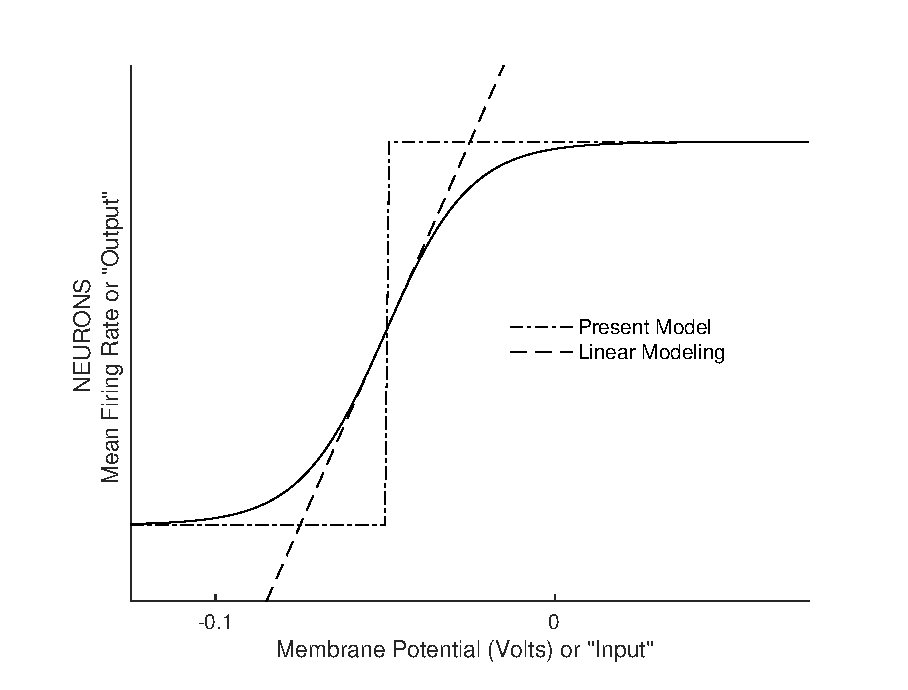
\includegraphics[width=0.75\textwidth]{Hopfield_Fig_1.eps}
		\caption{Firing rate versus membrane voltage for a typical neuron (solid line), dropping to 0 for large negative potentials and saturating for positive potentials. The broken lines show approximations used in modeling.}
		\label{fig:1}
	\end{figure}

	\begin{equation}
		\sum_{j} T_{ij}V_j
	\end{equation}
	
	\begin{equation}
		\Delta T_{ij} = [V_i(t) V_j(t)]_{\text{average}}
	\end{equation}
	
	\section{Studies of the collective behaviors of the model}
	\begin{equation}
		E = - \frac{1}{2} \sum_{i\neq j} \sum_{i\neq j} T_{ij}V_iV_j
	\end{equation}
	
	\begin{equation}
		\Delta E = - \Delta V_i \sum_{j \neq i} T_{ij}V_j
	\end{equation}
	
	\begin{equation}
		\ln M = - \sum p_i \ln p_i
	\end{equation}
	
	\begin{equation}
		P = \frac{1}{\sqrt{2 \pi \sigma^2}} \int_{N/2}^{\infty} e^{-x^2/2 \sigma^2} dx
	\end{equation}
	
	\begin{equation}
		\Delta T_{ij} = (2X_i -1)(2X_j -1) \quad i,j \leq k < N
	\end{equation}
	
	\begin{equation}
		\sum_{j=1}^{k} c_{ij} x_j
	\end{equation}
	
	\begin{equation}
		\Delta T_{ij} = A \sum_{s} (2V^{s+1}_i - 1)(2V^s_j - 1) 
	\end{equation}
	
	\section{Discussion}
	
	\section{Acknowledgments}
	The work at California Institute of Technology was supported in part by National Science Foundation Grant DMR-8107494. This is contribution no. 6580 from the Division of Chemistry and Chemical Engineering.
	
	\bibliographystyle{ieeetr}
	\bibliography{Hopfield-1982}
	
\end{document}